\subsection{Complementary filter}
A complementary filter is used to combine the measurement data from the accelerometer and gyros in the IMU. 
Data from the accelerometer is used to calculate an angle of the Cubli frame.
The gyroscope measurement is integrated to get the angle of the Cubli frame. Both measurements are done to find the change on the axis of movement of the Cubli.
The two angle measurements of the IMU are sent through a filter and then summed in order to get an angle of the Cubli frame. \fxnote{Make a proper sketch of the complementary filter, B}
\begin{figure}[H] 
	\centering
	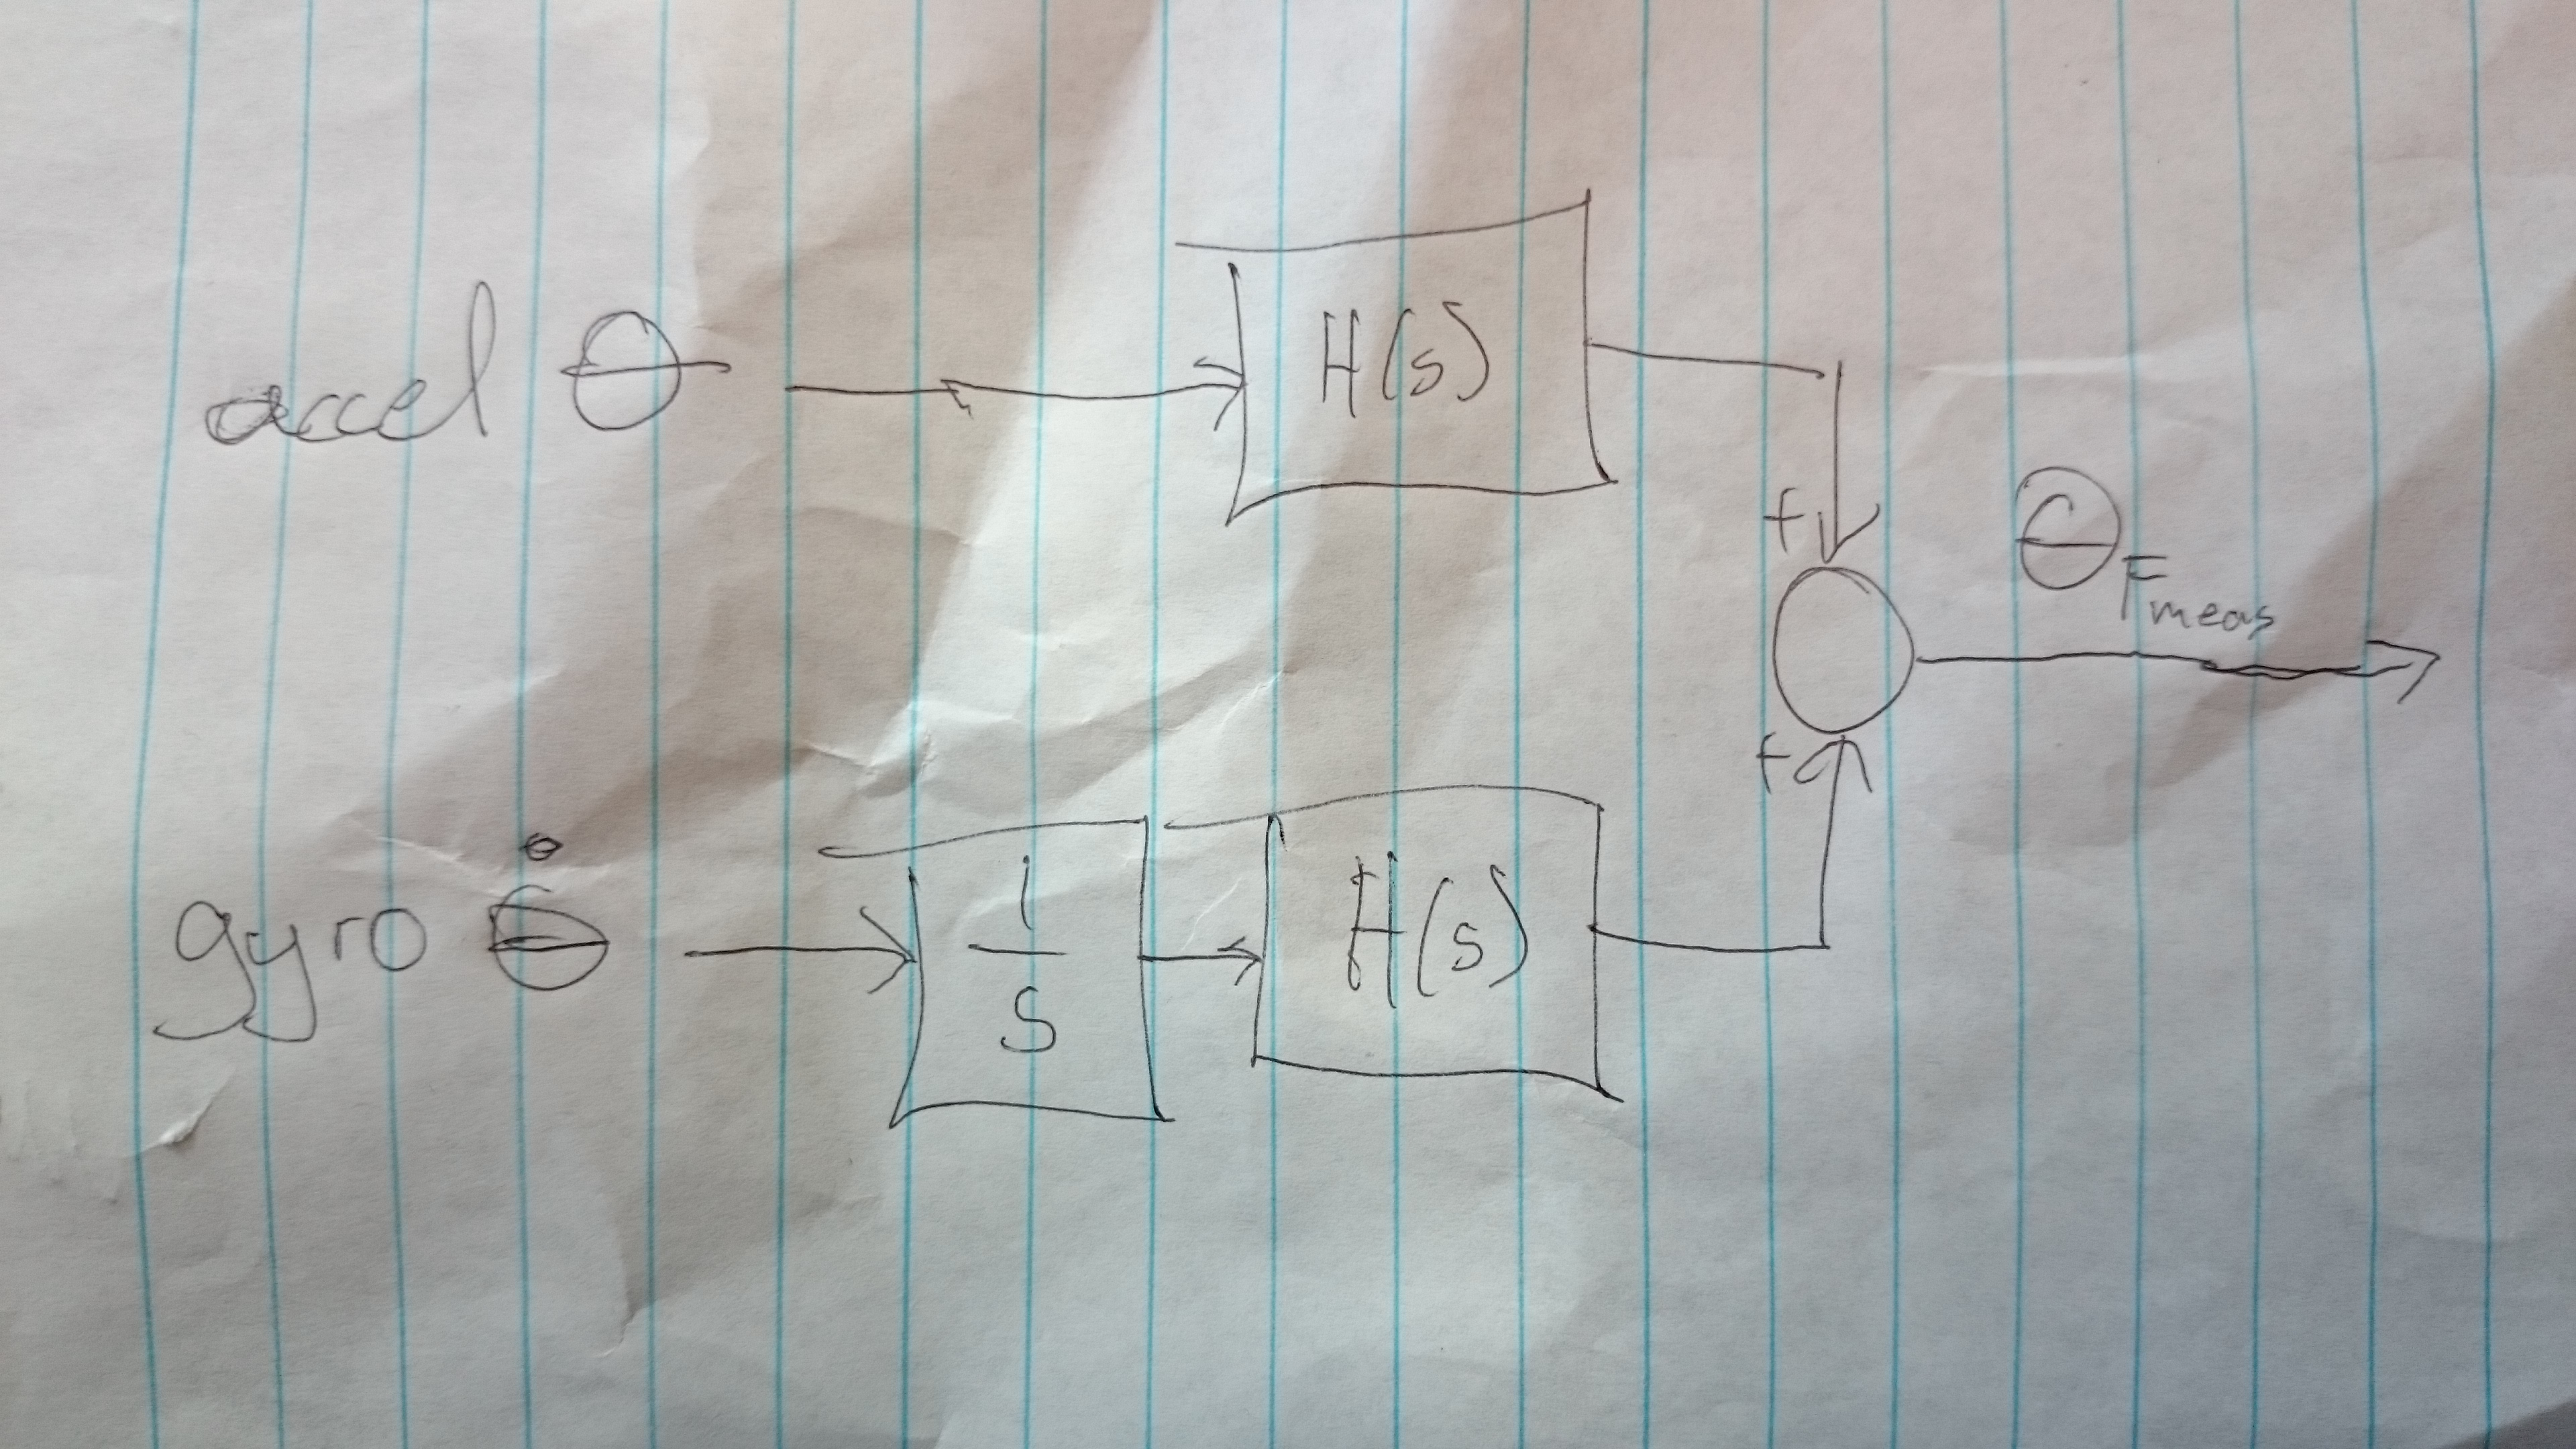
\includegraphics[scale=0.08]{figures/tempComplementaryFilter}
	\caption{Sketch of the structure of the complementary filter. Measurements from the accelerometer are calculated into an angle on the axis of movement. Data from gyro is used to find the angular velocity on the axis of movement}
	\label{blockComplementaryFilter}
\end{figure}
This is done to counteract drift of the gyroscope and error of the accelerometer.\fxnote{elaborate on the errors} 